%%%%%%%%%%%%%%%%%%%%%%%%%%%%%%%%%%%%%%%%%%%%%%%%%%%%%%%%%%%%%%%%%%%%%%%%%%%%%%%%
% Conference paper derived from the final undergraduate-thesis evidence.
%%%%%%%%%%%%%%%%%%%%%%%%%%%%%%%%%%%%%%%%%%%%%%%%%%%%%%%%%%%%%%%%%%%%%%%%%%%%%%%%

\documentclass[conference]{IEEEtran}
\IEEEoverridecommandlockouts

\usepackage{cite}
\usepackage{amsmath,amssymb,amsfonts}
\usepackage{graphicx}
\usepackage{textcomp}
\usepackage{xcolor}
\usepackage{booktabs}
\usepackage{multirow}
\usepackage{tabularx}
\usepackage{array}
\usepackage{balance}
\usepackage{tikz}
\usetikzlibrary{arrows.meta,positioning,calc}

\newcolumntype{Y}{>{\raggedright\arraybackslash}X}
\def\BibTeX{{\rm B\kern-.05em{\sc i\kern-.025em b}\kern-.08em
    T\kern-.1667em\lower.7ex\hbox{E}\kern-.125emX}}

\begin{document}

\title{Autonomous Excavator Control with\\
Deep Learning-Based Multi-Modal Perception}

\author{
\IEEEauthorblockN{
1\textsuperscript{st} Muhammad Aditya Rahmansyah Baskoro,\quad
2\textsuperscript{nd} Ahmad Ataka Awwalur Rizqi,\quad
3\textsuperscript{rd} Igi Ardiyanto}
\IEEEauthorblockA{
\textit{Department of Electrical Engineering and Information Technology}\\
\textit{Universitas Gadjah Mada}\\
Yogyakarta, Indonesia\\
\{muhammadadityarahmansyahbaskoro@mail.ugm.ac.id,\;
ahmad.ataka.ar@ugm.ac.id,\;
igi@ugm.ac.id\}}
}

\maketitle

\begin{abstract}
Autonomous excavator manipulation requires perception outputs that are not only detectable but metrically accurate enough to command the bucket. This paper presents an ego-centric camera--LiDAR perception system that estimates planar rubble and bin target centers in a simulated construction workspace. Six cameras are lifted into a bird's-eye-view (BEV) representation, a mast-mounted 64-beam LiDAR is encoded with PointPillars, and both features are combined by spatial gated fusion before center-based detection. The model is trained on 1,255 synthetic frames containing normal targets, target-like non-targets, and controlled sensor degradations. On the primary held-out test split, the fused model achieves 0.913 all-point mAP, 0.050\,m mean planar translation error, 0.084\,m P90 translation error, and 0.841 recall within the 0.25\,m task tolerance. Relative to a LiDAR-only model trained on the same data, fusion improves mAP from 0.871 to 0.913, bin AP from 0.773 to 0.844, and task-tolerance recall from 0.796 to 0.841, while metric localization remains essentially unchanged. Fusion also reduces false positives on target-like distractors from 77 to 22. In offline inverse-kinematics replay, fused perception supplies IK-compatible target pairs in 75.7\% of 74 kinematically eligible held-out scenes (56/74), compared with 67.6\% (50/74) for LiDAR-only perception. The 8.1-percentage-point increase mainly comes from additional usable bin targets. Under the tested sensor configuration, LiDAR retains metric localization accuracy, whereas the fused system improves target coverage and rejection of trained target-like negatives.
\end{abstract}

\begin{IEEEkeywords}
autonomous excavator, bird's-eye view, camera--LiDAR fusion, target localization, perception for control
\end{IEEEkeywords}

\section{Introduction}

Excavators are used for material handling, excavation, and pick-and-place in environments that are labor intensive and potentially hazardous for human operators \cite{xu2025construction,ataka2024icitee}. Existing automation research has demonstrated trajectory tracking, analytical control, and learned policies \cite{feng2018pid,jud2019trenching,egli2020iros,ataka2023icitee}. These methods address how an excavator should move once a target or trajectory is available. An autonomous manipulation system must additionally estimate that target from onboard sensors.

This distinction is important for pick-and-place. A 2D detection can indicate that an object exists, but the controller requires a metric target position. Camera observations provide dense visual and semantic information but do not directly measure depth. LiDAR provides metric geometry but can be sparse on small ground-level targets and cannot reliably distinguish geometrically similar target and non-target objects. The perception problem is therefore not simply object recognition: it is the estimation of task-relevant spatial state under complementary sensor limitations.

Camera--LiDAR fusion in autonomous driving commonly maps both modalities into a bird's-eye-view (BEV) representation \cite{liu2023bevfusion,liang2022bevfusion}. Camera features can be lifted into BEV using Lift-Splat-Shoot (LSS) \cite{philion2020lss}, while point clouds can be encoded efficiently with PointPillars \cite{lang2019pointpillars}. Center-based heads then predict object locations directly in metric BEV coordinates \cite{yin2021centerpoint}. However, excavator manipulation differs from road-scene detection in object scale, self-occlusion, sensor placement, and the tolerance with which a target must be localized. Existing excavator datasets also focus on terrain segmentation or other perception tasks rather than ego-centric 3D localization of work targets \cite{gooseex2024,agfusion2025}.

We study whether a compact BEV fusion system can provide control-relevant target centers for an excavator. Rather than treating fusion as uniformly beneficial, the evaluation separates detection, metric localization, semantic rejection, sensor degradation, and downstream target usability. The contributions are:

\begin{enumerate}
    \item An ego-centric BEV perception system and synthetic data pipeline for metric center estimation of rubble and bin targets using six cameras and a mast-mounted LiDAR.
    \item A task-conditioned evaluation protocol that combines all-point AP with translation-error tails and unconditional recall within a 0.25\,m manipulation tolerance.
    \item An empirical characterization of modality roles under the tested configuration: LiDAR retains metric localization accuracy, while the fused system improves target coverage and rejection of target-like non-targets.
    \item A scene-level IK replay showing that score-based selection from fused perception increases the proportion of eligible scenes supplied with an IK-compatible rubble--bin pair, followed by one representative perception-conditioned Gazebo execution.
\end{enumerate}

\section{Related Work}

\subsection{Excavator Automation and Perception}

Excavator automation has been approached through model-based control, trajectory generation, and reinforcement learning \cite{feng2018pid,zhang2019hybrid,jud2019trenching,egli2022ral}. Perception is often simplified through simulator state, prescribed trajectories, or image-level detection \cite{ataka2023icitee,ataka2024icitee,laksana2025ppo}. These studies establish that manipulation and motion control are feasible, but they do not directly characterize whether ego-centric multi-modal sensing can provide sufficiently accurate target centers.

Datasets closer to heavy equipment do not fully cover this problem. GOOSE-Ex provides excavator-mounted camera and LiDAR data for semantic terrain understanding \cite{gooseex2024}. Excavator3D focuses on different object definitions and sensing objectives \cite{agfusion2025}. Consequently, a task-specific synthetic pipeline is used here to control geometry, annotations, visibility, and target-like negatives.

\subsection{BEV Multi-Modal Detection}

BEV representations provide a common metric plane for heterogeneous sensors. LSS associates image features with a predicted depth distribution before projecting them into BEV \cite{philion2020lss}. PointPillars converts sparse point clouds into a pseudo-image suitable for 2D convolution \cite{lang2019pointpillars}. BEVFusion demonstrates that camera and LiDAR features can be combined in a unified BEV space \cite{liu2023bevfusion,liang2022bevfusion}, while CenterPoint formulates 3D detection around object centers \cite{yin2021centerpoint}. Our system adopts these principles but reduces the learned output contract to target class, confidence, and planar BEV center.

\subsection{Perception Evaluation for Downstream Tasks}

Autonomous-driving research has increasingly evaluated perception in relation to planning rather than only standalone detection scores \cite{hu2023uniad}. The same principle is relevant to manipulation: mean error over matched detections does not penalize missed objects and can hide tail failures. We therefore report all-point AP for ranking quality, translation-error percentiles for matched predictions, and recall within a task tolerance over all ground-truth objects.

\section{System and Method}

\subsection{Task, Simulation, and Sensors}

The task consists of selecting one rubble target for reaching and one bin target for placement. Each perception output contains a learned planar center $(c_x,c_y)$, class $k$, and confidence score $s$. Target height is supplied by a class prior. A rubble prediction is considered within task tolerance when its planar center error is below $d_{\mathrm{task}}=0.25$\,m.

The environment is implemented in ROS~2 Humble and Gazebo Fortress \cite{ros2humble,gazebofortress}. The simulated excavator has five articulated degrees of freedom. Six RGB cameras provide overlapping 360-degree visual coverage at 640$\times$360 pixels and 5\,Hz; images are resized to 448$\times$256 for training. A 64-beam LiDAR is mounted at $(0,0.15,3.25)$\,m relative to the cabin, with 1,024 horizontal samples, a 360-degree horizontal field of view, and 10\,Hz sampling. The model uses RGB and LiDAR; simulator depth cameras are retained only for auditing.

Scenes vary the number, geometry, and position of targets, arm pose, and self-occlusion. Controlled training perturbations include image darkening, camera dropout, random LiDAR thinning, and LiDAR sector dropout. Target-like non-target objects are included as unlabeled hard negatives. The final unified training set contains 1,255 frames, 4,853 target instances, and 680 target-like distractors; validation contains 264 frames, 1,047 targets, and 170 distractors. Splits are separated by episode.

\subsection{BEV Perception Architecture}

\begin{figure*}[t]
\centering
\resizebox{0.96\textwidth}{!}{%
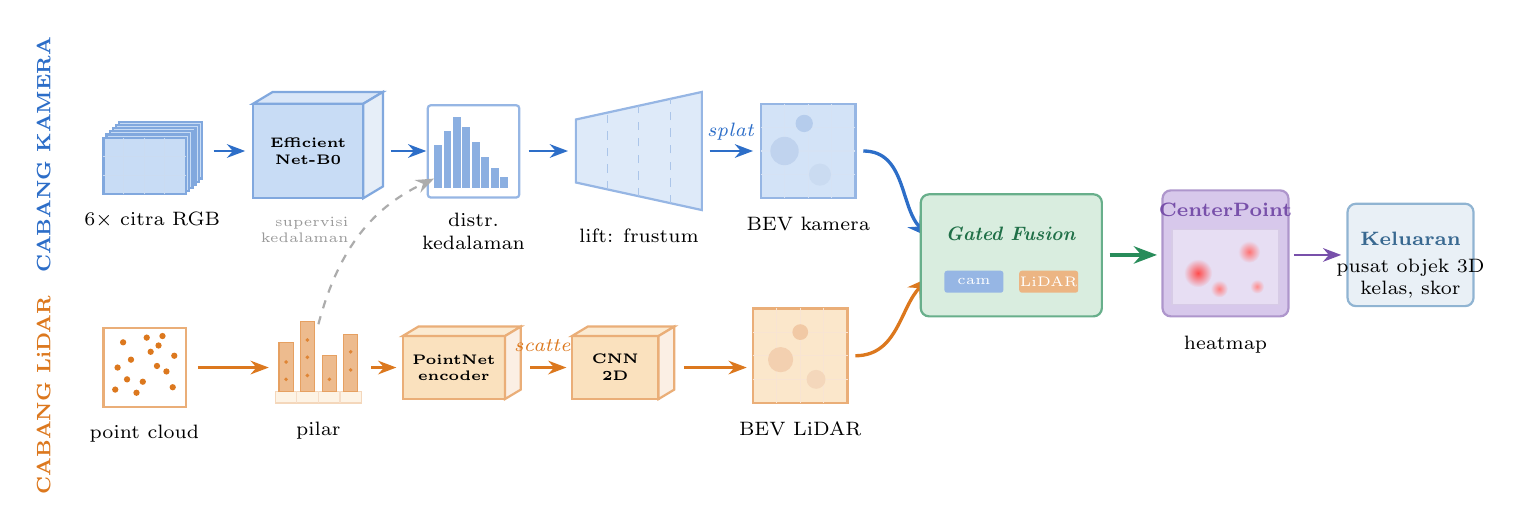
\begin{tikzpicture}[font=\small,>=Stealth]

  % -- colour palette --
  \definecolor{camblue}{RGB}{45,110,200}
  \definecolor{camlight}{RGB}{200,220,245}
  \definecolor{lidarorange}{RGB}{220,120,30}
  \definecolor{lidarlight}{RGB}{250,225,190}
  \definecolor{bevgreen}{RGB}{40,140,90}
  \definecolor{fusiongreen}{RGB}{160,210,175}
  \definecolor{headpurple}{RGB}{120,80,170}
  \definecolor{headlight}{RGB}{215,200,235}
  \definecolor{outblue}{RGB}{70,130,180}

  % =====================================================================
  %  CAMERA BRANCH (top row)
  % =====================================================================

  % --- 6× stacked camera images ---
  \foreach \i/\sh in {5/0.20, 4/0.16, 3/0.12, 2/0.08, 1/0.04, 0/0.00}{
    \fill[camlight,draw=camblue!60,thick]
      ($(0.0+\sh, 2.6+\sh)$) rectangle ++(1.05,0.72);
  }
  \foreach \x in {0.26,0.52,0.78}
    \draw[camblue!25] (\x,2.6) -- (\x,3.32);
  \foreach \y in {2.84,3.08}
    \draw[camblue!25] (0,\y) -- (1.05,\y);
  \node[below,font=\scriptsize,align=center] at (0.62,2.50)
    {6$\times$ citra RGB};

  % --- arrow ---
  \draw[->,thick,camblue] (1.40,3.15) -- (1.80,3.15);

  % --- EfficientNet-B0 backbone (3D tensor block, widened to fit text perfectly) ---
  \fill[camlight,draw=camblue!60,thick]
    (1.90,2.55) -- (3.30,2.55) -- (3.30,3.75) -- (1.90,3.75) -- cycle;
  \fill[camlight!70!white,draw=camblue!60,thick]
    (1.90,3.75) -- (3.30,3.75) -- (3.55,3.90) -- (2.15,3.90) -- cycle;
  \fill[camblue!12,draw=camblue!60,thick]
    (3.30,2.55) -- (3.30,3.75) -- (3.55,3.90) -- (3.55,2.70) -- cycle;
  \node[font=\tiny\bfseries,align=center] at (2.60,3.15) {Efficient\\Net-B0};

  % --- arrow ---
  \draw[->,thick,camblue] (3.65,3.15) -- (4.10,3.15);

  % --- Depth distribution (discrete bins) ---
  \begin{scope}[shift={(4.20,2.68)}]
    \fill[white,draw=camblue!50,thick,rounded corners=1pt]
      (-0.08,-0.12) rectangle (1.08,1.05);
    \foreach \x/\h in {0.00/0.55, 0.12/0.72, 0.24/0.90, 0.36/0.78,
                        0.48/0.58, 0.60/0.40, 0.72/0.25, 0.84/0.14}{
      \fill[camblue!55] (\x,0) rectangle ++(0.10,\h);
    }
    \node[below,font=\scriptsize,align=center] at (0.50,-0.20)
      {distr.\\kedalaman};
  \end{scope}

  % --- arrow ---
  \draw[->,thick,camblue] (5.40,3.15) -- (5.90,3.15);

  % --- LSS frustum (3D wedge with depth slices) ---
  \begin{scope}[shift={(6.00,2.50)}]
    \fill[camlight!60,draw=camblue!50,thick]
      (0.0, 0.25) -- (1.60,-0.10) -- (1.60,1.40) -- (0.0, 1.05) -- cycle;
    \foreach \t in {0.25,0.50,0.75}{
      \draw[camblue!40,dashed]
        ($(0.0,0.25)!\t!(1.60,-0.10)$) -- ($(0.0,1.05)!\t!(1.60,1.40)$);
    }
    \node[below,font=\scriptsize,align=center] at (0.80,-0.22)
      {lift: frustum};
  \end{scope}

  % --- arrow (splat) ---
  \draw[->,thick,camblue] (7.70,3.15) -- (8.25,3.15)
    node[midway,above,font=\scriptsize]{\textit{splat}};

  % --- Camera BEV feature map ---
  \begin{scope}[shift={(8.35,2.55)}]
    \fill[camlight!80] (0,0) rectangle (1.20,1.20);
    \draw[camblue!50,thick] (0,0) rectangle (1.20,1.20);
    \foreach \x in {0.3,0.6,0.9} \draw[camblue!20] (\x,0)--(\x,1.20);
    \foreach \y in {0.3,0.6,0.9} \draw[camblue!20] (0,\y)--(1.20,\y);
    \fill[camblue!30] (0.3,0.6) circle (0.18);
    \fill[camblue!25] (0.75,0.30) circle (0.14);
    \fill[camblue!35] (0.55,0.95) circle (0.11);
    \node[below,font=\scriptsize,align=center] at (0.60,-0.12)
      {BEV kamera};
  \end{scope}

  % =====================================================================
  %  LIDAR BRANCH (bottom row)
  % =====================================================================

  % --- Point cloud ---
  \begin{scope}[shift={(0.0,0.0)}]
    \draw[lidarorange!60,thick] (0,-0.10) rectangle (1.05,0.90);
    \foreach \p in {(0.15,0.12),(0.35,0.50),(0.50,0.22),(0.70,0.68),
                    (0.25,0.72),(0.80,0.35),(0.55,0.78),(0.90,0.55),
                    (0.42,0.08),(0.68,0.42),(0.18,0.40),(0.88,0.15),
                    (0.60,0.60),(0.30,0.25),(0.75,0.80)}
      \fill[lidarorange] \p circle (0.04);
    \node[below,font=\scriptsize,align=center] at (0.52,-0.20)
      {point cloud};
  \end{scope}

  % --- arrow ---
  \draw[->,thick,lidarorange] (1.20,0.40) -- (2.10,0.40);

  % --- Pillarization ---
  \begin{scope}[shift={(2.18,-0.05)}]
    \fill[lidarlight!40] (0,0) rectangle (1.10,0.15);
    \draw[lidarorange!30] (0,0) rectangle (1.10,0.15);
    \foreach \x in {0.275,0.55,0.825} \draw[lidarorange!25] (\x,0)--(\x,0.15);
    \foreach \x/\h in {0.05/0.62, 0.32/0.88, 0.60/0.45, 0.87/0.72}{
      \fill[lidarorange!50] (\x,0.15) rectangle ++(0.18,\h);
      \draw[lidarorange!70] (\x,0.15) rectangle ++(0.18,\h);
    }
    \foreach \p in {(0.14,0.30),(0.14,0.52),(0.41,0.35),(0.41,0.58),
                    (0.41,0.80),(0.69,0.30),(0.96,0.42),(0.96,0.65)}
      \fill[lidarorange!90] \p circle(0.025);
    \node[below,font=\scriptsize,align=center] at (0.55,-0.12)
      {pilar};
  \end{scope}

  % --- arrow ---
  \draw[->,thick,lidarorange] (3.40,0.40) -- (3.72,0.40);

  % --- PointNet encoder (3D tensor block, widened to fit text perfectly) ---
  \fill[lidarlight,draw=lidarorange!60,thick]
    (3.80,0.0) -- (5.10,0.0) -- (5.10,0.80) -- (3.80,0.80) -- cycle;
  \fill[lidarlight!70!white,draw=lidarorange!60,thick]
    (3.80,0.80) -- (5.10,0.80) -- (5.30,0.92) -- (4.00,0.92) -- cycle;
  \fill[lidarorange!12,draw=lidarorange!60,thick]
    (5.10,0.0) -- (5.10,0.80) -- (5.30,0.92) -- (5.30,0.12) -- cycle;
  \node[font=\tiny\bfseries,align=center] at (4.45,0.40) {PointNet\\encoder};

  % --- arrow (scatter) ---
  \draw[->,thick,lidarorange] (5.42,0.40) -- (5.88,0.40)
    node[midway,above=2pt,font=\scriptsize]{\textit{scatter}};

  % --- CNN 2D (3D tensor block, widened to fit text perfectly) ---
  \fill[lidarlight,draw=lidarorange!60,thick]
    (5.95,0.0) -- (7.05,0.0) -- (7.05,0.80) -- (5.95,0.80) -- cycle;
  \fill[lidarlight!70!white,draw=lidarorange!60,thick]
    (5.95,0.80) -- (7.05,0.80) -- (7.25,0.92) -- (6.15,0.92) -- cycle;
  \fill[lidarorange!12,draw=lidarorange!60,thick]
    (7.05,0.0) -- (7.05,0.80) -- (7.25,0.92) -- (7.25,0.12) -- cycle;
  \node[font=\tiny\bfseries,align=center] at (6.50,0.40) {CNN\\2D};

  % --- arrow ---
  \draw[->,thick,lidarorange] (7.37,0.40) -- (8.17,0.40);

  % --- LiDAR BEV feature map ---
  \begin{scope}[shift={(8.25,-0.05)}]
    \fill[lidarlight!80] (0,0) rectangle (1.20,1.20);
    \draw[lidarorange!60,thick] (0,0) rectangle (1.20,1.20);
    \foreach \x in {0.3,0.6,0.9} \draw[lidarorange!20] (\x,0)--(\x,1.20);
    \foreach \y in {0.3,0.6,0.9} \draw[lidarorange!20] (0,\y)--(1.20,\y);
    \fill[lidarorange!35] (0.35,0.55) circle (0.16);
    \fill[lidarorange!30] (0.80,0.30) circle (0.12);
    \fill[lidarorange!40] (0.60,0.90) circle (0.10);
    \node[below,font=\scriptsize,align=center] at (0.60,-0.12)
      {BEV LiDAR};
  \end{scope}

  % =====================================================================
  %  GATED FUSION
  % =====================================================================

  \draw[->,thick,camblue,line width=1.2pt]
    (9.65,3.15) to[out=0,in=135] (10.50,2.05);
  \draw[->,thick,lidarorange,line width=1.2pt]
    (9.55,0.55) to[out=0,in=225] (10.50,1.55);

  \begin{scope}[shift={(10.38,1.05)}]
    \fill[fusiongreen!40,draw=bevgreen!70,thick,rounded corners=3pt]
      (0,0) rectangle (2.30,1.55);
    \node[font=\scriptsize\bfseries,bevgreen!80!black] at (1.15,1.05)
      {\textit{Gated Fusion}};
    % gate bar
    \fill[camblue!50,rounded corners=1pt] (0.30,0.30) rectangle ++(0.75,0.28);
    \fill[lidarorange!55,rounded corners=1pt] (1.25,0.30) rectangle ++(0.75,0.28);
    \node[font=\tiny,white] at (0.675,0.44) {cam};
    \node[font=\tiny,white] at (1.625,0.44) {LiDAR};
  \end{scope}

  % --- arrow ---
  \draw[->,thick,bevgreen,line width=1.2pt] (12.78,1.83) -- (13.38,1.83);

  % =====================================================================
  %  CENTERPOINT HEAD
  % =====================================================================

  \begin{scope}[shift={(13.45,1.05)}]
    \fill[headlight,draw=headpurple!60,thick,rounded corners=3pt]
      (0,0) rectangle (1.60,1.60);
    \node[font=\scriptsize\bfseries,headpurple] at (0.80,1.35)
      {CenterPoint};
    \fill[headlight!60] (0.12,0.15) rectangle (1.48,1.10);
    \draw[headpurple!30] (0.12,0.15) rectangle (1.48,1.10);
    \shade[inner color=red!70,outer color=headlight!60]
      (0.45,0.55) circle (0.18);
    \shade[inner color=red!55,outer color=headlight!60]
      (1.10,0.82) circle (0.14);
    \shade[inner color=red!50,outer color=headlight!60]
      (0.72,0.35) circle (0.11);
    \shade[inner color=red!45,outer color=headlight!60]
      (1.20,0.38) circle (0.09);
    \node[below,font=\scriptsize,align=center] at (0.80,-0.12)
      {heatmap};
  \end{scope}

  % --- arrow ---
  \draw[->,thick,headpurple] (15.12,1.83) -- (15.72,1.83);

  % =====================================================================
  %  OUTPUT
  % =====================================================================

  \begin{scope}[shift={(15.80,1.18)}]
    \fill[outblue!12,draw=outblue!60,thick,rounded corners=3pt]
      (0,0) rectangle (1.60,1.30);
    \node[font=\scriptsize\bfseries,outblue!80!black,align=center] at (0.80,0.85)
      {Keluaran};
    \node[font=\scriptsize,align=center] at (0.80,0.35)
      {pusat objek 3D\\kelas, skor};
  \end{scope}

  % =====================================================================
  %  BRANCH LABELS
  % =====================================================================

  \node[font=\scriptsize\bfseries,camblue,rotate=90,anchor=south] at (-0.55,3.10)
    {CABANG KAMERA};
  \node[font=\scriptsize\bfseries,lidarorange,rotate=90,anchor=south] at (-0.55,0.05)
    {CABANG LiDAR};

  % =====================================================================
  %  DEPTH SUPERVISION (dashed LiDAR → camera depth)
  % =====================================================================
  \draw[dashed,gray!65,thick,->] (2.73,0.95) to[out=75,in=205]
    node[pos=0.55,left=2pt,font=\tiny,gray!80,align=right]
    {supervisi\\kedalaman} (4.20,2.80);

\end{tikzpicture}%
}
\caption{Final perception architecture. Camera and LiDAR features are encoded independently, aligned in a common metric BEV grid, combined by a spatial gate, and decoded as task-relevant object centers.}
\label{fig:architecture}
\end{figure*}

Each image is encoded by a shared EfficientNet-B0 backbone \cite{tan2019efficientnet}. LSS predicts 64 depth bins over 0.5--15\,m and projects image features into a 256$\times$256 BEV grid covering a 20$\times$20\,m workspace. LiDAR points are encoded by PointPillars into the same grid. The resulting cell size is 0.078\,m, finer than the 0.25\,m task tolerance.

Camera and LiDAR BEV features are projected to a common channel dimension and combined using a spatial gate:
\begin{align}
    \mathbf{g} &=
    \sigma\!\left(\mathrm{Conv}\left[
    \mathbf{F}_{\mathrm{cam}};\mathbf{F}_{\mathrm{lid}}
    \right]\right),\\
    \mathbf{F}_{\mathrm{fused}} &=
    \mathbf{g}\odot\mathbf{F}_{\mathrm{cam}}
    +(1-\mathbf{g})\odot\mathbf{F}_{\mathrm{lid}}.
\end{align}
A simplified CenterPoint-style head predicts two class heatmaps and sub-cell offsets. The evaluated translation error is planar; target height is assigned from the class mean. Full box dimensions and yaw are omitted because the downstream contract requires target positions rather than complete oriented 3D boxes.

\subsection{Training and Evaluation}

The fused and LiDAR-only models are trained on the same unified data. The fused model has 10.58 million parameters and the LiDAR-only model approximately 1.1 million. Both are optimized with AdamW \cite{loshchilov2019decoupled} for 16 epochs using a learning rate of $2\times10^{-5}$ and an effective batch size of eight. The loss combines Gaussian focal loss for center heatmaps, Smooth-L1 offset loss, and sparse pseudo-depth supervision for the camera branch.

Predictions are matched one-to-one by class and planar center distance using a 1.0\,m detection radius. Detector quality is reported with all-point AP over the full confidence ranking. Operating metrics are reported at a validation-selected score threshold of 0.60. For ground-truth object $j$, let $m(j)$ denote its same-class matched prediction, when one exists. The planar center error and unconditional recall within tolerance $\tau$ are
\begin{align}
    e_j &=
    \left\|
    \hat{\mathbf{c}}_{m(j)}-\mathbf{c}_j
    \right\|_2,\\
    R_{\tau} &=
    \frac{1}{N_{\mathrm{GT}}}
    \sum_{j=1}^{N_{\mathrm{GT}}}
    \mathbb{1}\!\left[
    m(j)\ \text{exists}\ \land\ e_j<\tau
    \right].
    \label{eq:r025}
\end{align}
Thus, R@0.25 is $R_{\tau}$ at $\tau=0.25$\,m; missed objects contribute zero. mATE and P90 ATE summarize $e_j$ only over existing matches. The primary test split contains 150 frames, 360 rubble objects, and 218 bins.

To determine whether learned localization merely copies raw geometry, we also compute an oracle centroid from LiDAR points inside each ground-truth box. Ground-truth association intentionally removes detection as a confound and gives the geometric estimator an advantageous comparison. Robustness is evaluated by removing or degrading individual modalities without retraining.

For the downstream evaluation, let $\mathcal{E}$ be the set of scenes whose ground truth contains at least one IK-reachable rubble and bin from the fixed base pose. The primary selector uses no ground truth: at the 0.60 operating threshold, it chooses the highest-scoring IK-reachable prediction for each class. Let $C_k(s)\in\{0,1\}$ indicate that the selected prediction for class $k$ exists and lies within its class tolerance of a valid target in scene $s$. The scene-level compatible-pair rate is
\begin{equation}
    R_{\mathrm{pair}}^{\mathrm{IK}}
    =
    \frac{1}{|\mathcal{E}|}
    \sum_{s\in\mathcal{E}}
    C_{\mathrm{rubble}}(s)
    C_{\mathrm{bin}}(s),
    \label{eq:ik_pair_rate}
\end{equation}
using tolerances of 0.25\,m for rubble and 0.30\,m for bins. This score-based replay is the quantitative result; one held-out scene is subsequently executed in Gazebo only as a qualitative integration example.

\section{Results}

\subsection{Main Perception Result}

Table~\ref{tab:main} reports the final models on the primary held-out split. On these trained checkpoints, fusion increases all-point mAP by 0.042, bin AP by 0.071, operating recall by 0.052, and R@0.25 by 0.045. In contrast, mATE and P90 are nearly unchanged. The central result is therefore not that fusion replaces LiDAR geometry; it increases the set of correctly detected targets within task tolerance while preserving the metric accuracy retained by the LiDAR branch. Each architecture is represented by one training run, so the deltas are empirical comparisons on this test set rather than estimates of variation across training seeds.

\begin{table}[t]
\caption{Final perception performance on the primary held-out test split. AP is all-point AP; operating metrics use a score threshold of 0.60.}
\label{tab:main}
\centering
\scriptsize
\setlength{\tabcolsep}{2.6pt}
\begin{tabular}{lcccccc}
\toprule
\textbf{Model} & \textbf{mAP} & \textbf{Bin AP} &
\textbf{Recall} & \textbf{mATE} & \textbf{P90} & \textbf{R@.25} \\
\midrule
LiDAR-only & 0.871 & 0.773 & 0.798 & \textbf{0.047} & \textbf{0.083} & 0.796 \\
Fusion & \textbf{0.913} & \textbf{0.844} & \textbf{0.850} & 0.050 & 0.084 & \textbf{0.841} \\
\bottomrule
\end{tabular}
\end{table}

The class-level result reveals a coverage--localization trade-off. For bins, fusion increases R@0.25 from 0.628 to 0.729, but P90 ATE increases from 0.062 to 0.103\,m. Fusion admits more difficult bins rather than improving the localization tail of already well-observed bins. Under this configuration, the fused model broadens coverage while the LiDAR branch retains the strongest metric tail.

\subsection{Does Learning Matter Beyond Sensor Geometry?}

The oracle centroid comparison in Table~\ref{tab:geometry} tests whether accurate sensing alone explains the result. For bins, the raw centroid has a P90 error of 0.383\,m and R@0.25 of 0.431, despite receiving the correct ground-truth association. The learned LiDAR BEV model reaches a P90 of 0.062\,m. A deployable classical clustering baseline is substantially weaker still, with approximately 0.012 mAP and 0.659\,m P90 ATE. The result is consistent with learned association and center inference beyond raw point averaging. Because the centroid and learned metrics are not a fully paired same-object estimator comparison, the table is not used to quantify a causal estimator gain.

\begin{table}[t]
\caption{Raw geometry and learned center estimation.}
\label{tab:geometry}
\centering
\small
\begin{tabular}{llcc}
\toprule
\textbf{Class} & \textbf{Estimator} & \textbf{P90 (m)} & \textbf{R@0.25} \\
\midrule
\multirow{3}{*}{Rubble}
 & GT-box centroid & 0.156 & \textbf{0.944} \\
 & LiDAR BEV & 0.088 & 0.897 \\
 & Fused BEV & \textbf{0.083} & 0.908 \\
\midrule
\multirow{3}{*}{Bin}
 & GT-box centroid & 0.383 & 0.431 \\
 & LiDAR BEV & \textbf{0.062} & 0.628 \\
 & Fused BEV & 0.103 & \textbf{0.729} \\
\bottomrule
\end{tabular}
\end{table}

\subsection{What Camera--LiDAR Fusion Adds}

Target-like non-targets test whether the complete fused system improves target selection relative to the LiDAR-only baseline. At the same 0.60 threshold, LiDAR-only produces 188 target true positives and 77 distractor false positives. Fusion produces 195 target true positives and only 22 distractor false positives, increasing target precision from 0.709 to 0.886. This result depends on including representative hard negatives during training; it should not be interpreted as zero-shot semantic rejection. Because the models also differ in capacity and auxiliary camera training, this is a system-level comparison rather than perfect causal isolation of visual semantics.

\begin{table}[t]
\caption{Target and distractor attribution on the semantic test.}
\label{tab:semantic}
\centering
\small
\begin{tabular}{lrrrr}
\toprule
\textbf{Model} & \textbf{TP} & \textbf{Distr. FP} & \textbf{Prec.} & \textbf{Recall} \\
\midrule
LiDAR-only & 188 & 77 & 0.709 & 0.767 \\
Fusion & \textbf{195} & \textbf{22} & \textbf{0.886} & \textbf{0.796} \\
\bottomrule
\end{tabular}
\end{table}

The modality counterfactuals in Table~\ref{tab:robustness} provide a second view. Removing cameras preserves a low P90 but decreases R@0.25 from 0.841 to 0.758. Removing LiDAR retains substantial AP but increases P90 to 0.297\,m and reduces R@0.25 to 0.413. Therefore, camera-only evidence can retain object awareness but is not sufficiently metric for direct action in this system. Under severe random LiDAR thinning, the robustly trained fused model degrades without catastrophic collapse.

\begin{table}[t]
\caption{Counterfactual sensor evaluation of the final fused model.}
\label{tab:robustness}
\centering
\scriptsize
\setlength{\tabcolsep}{4pt}
\begin{tabular}{lccc}
\toprule
\textbf{Condition} & \textbf{mAP} & \textbf{R@0.25} & \textbf{P90 (m)} \\
\midrule
Normal & \textbf{0.913} & \textbf{0.841} & 0.084 \\
Camera removed & 0.866 & 0.758 & \textbf{0.077} \\
LiDAR removed & 0.812 & 0.413 & 0.297 \\
LiDAR retained at 10\% & 0.887 & 0.718 & 0.164 \\
Camera darkened & 0.854 & 0.722 & 0.076 \\
\bottomrule
\end{tabular}
\end{table}

\subsection{Observability Boundary}

Figure~\ref{fig:observability} summarizes the direct empirical boundary from per-object LiDAR support. Of 578 targets in the primary test split, 50 receive no LiDAR points and have zero R@0.25 at the operating threshold. The two small low-count groups are combined: R@0.25 is 0.429 for objects with 1--9 points, 0.874 for 10--29 points, and 0.948 for at least 30 points. These numerical bins are specific to the simulated sensor configuration, but the ordering is clear: metric target usability increases with local geometric evidence.

\begin{figure}[t]
\centering
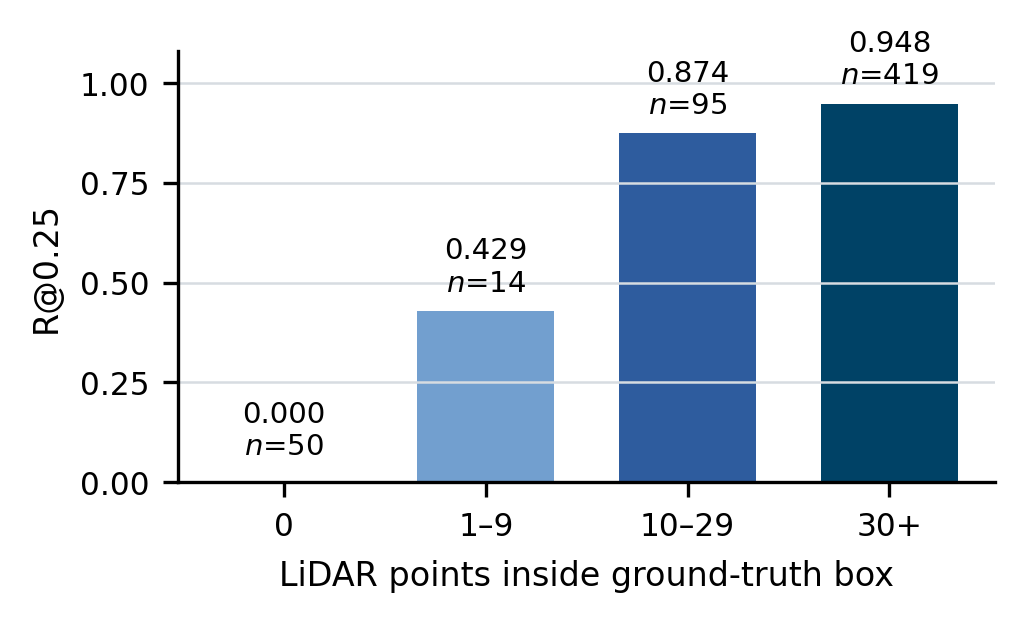
\includegraphics[width=\columnwidth]{figures/fig_3_lidar_support.png}
\caption{Task-tolerance recall increases with local LiDAR support. Counts above bars show the number of ground-truth objects in each stratum; the numerical thresholds are specific to the simulated sensor configuration.}
\label{fig:observability}
\end{figure}

\subsection{Perception-to-Control Replay}

The final evaluation asks whether object-level gains create usable task targets. Only scenes that contain at least one IK-reachable ground-truth rubble and bin are included; unreachable scenes require base repositioning and are not counted as perception failures. A simple selection rule chooses the highest-score IK-reachable prediction for each class. A replay is counted as IK-compatible when the selected rubble is within 0.25\,m and the selected bin within 0.30\,m of a valid target.

Among 150 held-out frames, 74 are kinematically eligible under ground-truth reachability. Fusion yields IK-compatible selections in 75.7\% of these scenes (56/74), compared with 67.6\% (50/74) for LiDAR-only. Rubble reach compatibility is identical at 94.6\%; the difference comes from place compatibility, which increases from 70.3\% to 81.1\%. Missing bin candidates decrease from 22 to 12, showing that the 8.1-percentage-point task-level gain primarily comes from additional usable bin estimates.

\begin{table}[t]
\caption{Offline IK replay on kinematically eligible held-out scenes.}
\label{tab:ik}
\centering
\scriptsize
\setlength{\tabcolsep}{2.2pt}
\begin{tabular}{lccc}
\toprule
\textbf{Model} & \textbf{\shortstack{IK-pair\\rate}} & \textbf{Reach} & \textbf{Place} \\
\midrule
LiDAR-only & 67.6\% (50/74) & \textbf{94.6\%} & 70.3\% \\
Fusion & \textbf{75.7\% (56/74)} & \textbf{94.6\%} & \textbf{81.1\%} \\
\bottomrule
\end{tabular}
\end{table}

\begin{figure}[t]
\centering
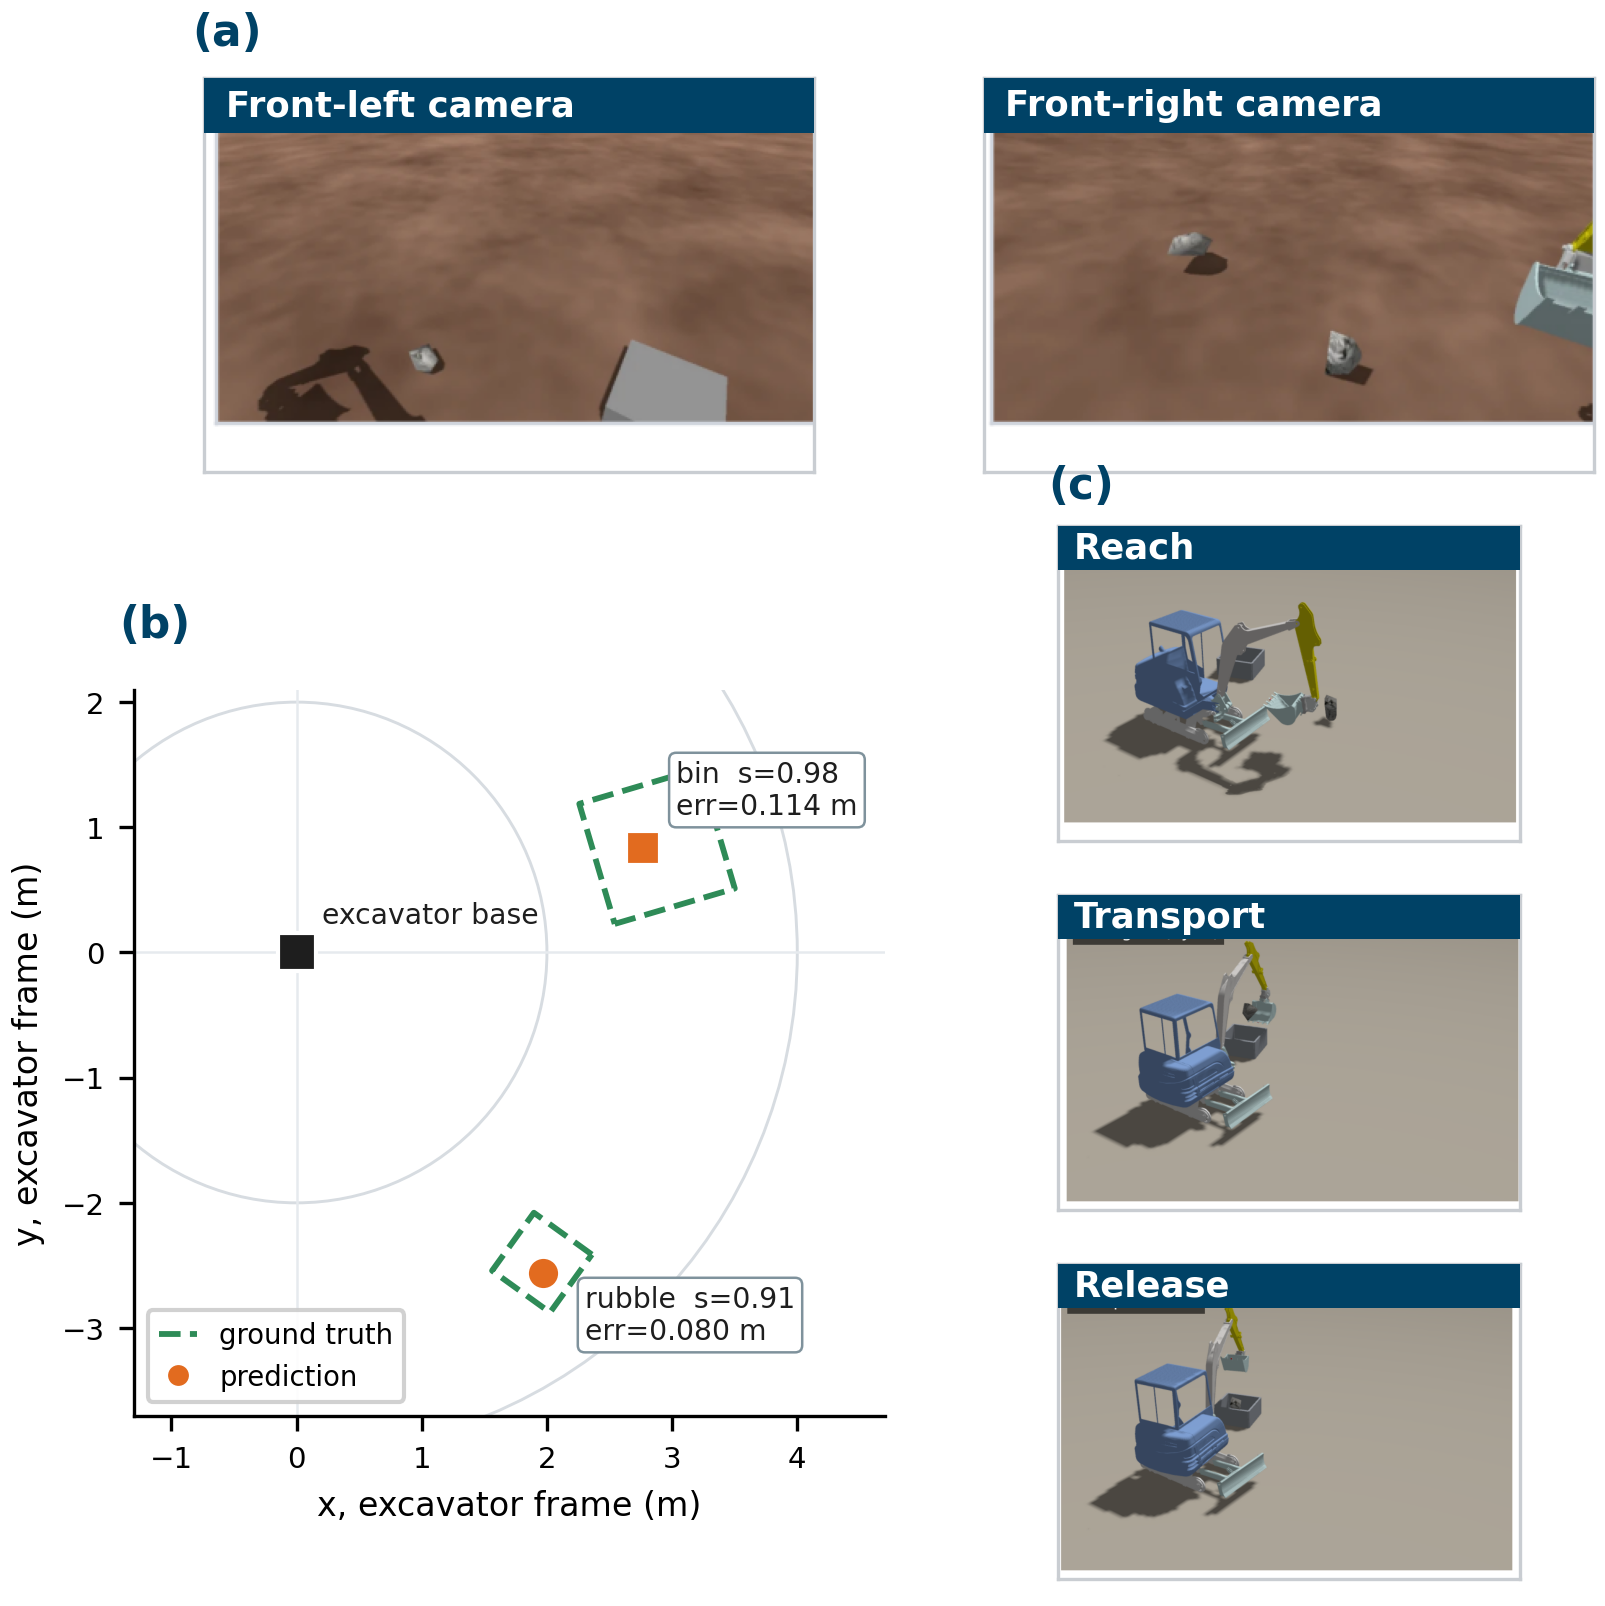
\includegraphics[width=\columnwidth]{figures/fig_2_perception_to_action.png}
\caption{Representative perception-to-action trace: (a) selected camera observations, (b) target estimates on the LiDAR BEV, and (c) reach, transport, and release. Targets come from predictions only; reported rubble/bin errors are 0.080/0.114\,m.}
\label{fig:perception_to_action}
\end{figure}

Figure~\ref{fig:perception_to_action} shows one representative held-out scene executed in Gazebo using prediction-selected targets only. The selected rubble and bin errors were 0.080\,m and 0.114\,m, respectively, and the released rubble settled 0.109\,m from the bin center. Perception ran once before motion, and transport used a kinematic attachment abstraction; therefore, this trace demonstrates interface continuity from sensing to motion but is not a success-rate or closed-loop manipulation result.

\section{Discussion}

The experiments support a simple system interpretation. First, the sensor configuration must provide local metric evidence. Second, learned BEV inference must associate evidence and estimate object centers; raw point centroids are not sufficient. Third, the fused system contributes where visual context is informative: recovering additional targets and rejecting trained target-like negatives. Finally, detections must be judged against task tolerance rather than AP alone.

This interpretation avoids two overclaims. Fusion does not improve every metric: LiDAR-only slightly outperforms fusion on the localization tail for bins that it already detects. Conversely, LiDAR is not a complete replacement for fusion: it misses more bins, rejects target-like non-targets less effectively, and supplies fewer usable place targets to IK. The meaningful comparison is therefore not which modality ``wins,'' but which system capability each modality supports.

The work has five principal limitations. All data are synthetic, so sim-to-real transfer is untested. The model operates on single frames and cannot actively reobserve uncertain targets. Only rubble and bin classes are evaluated. The downstream experiment consists of offline one-shot replay plus one representative Gazebo execution using kinematic attachment; it is not closed-loop physical excavation and does not model granular scooping, repeated observation during motion, or real hydraulic dynamics. Finally, each reported model is one trained checkpoint, so variation across random training seeds is not measured. These limits constrain the scope of the result but do not change the measured distinction between detection coverage, metric localization, and task-level target supply.

\section{Conclusion}

This paper presented an ego-centric camera--LiDAR BEV perception system for simulated excavator manipulation. The final fused model achieves 0.913 all-point mAP and 0.841 recall within a 0.25\,m task tolerance, while maintaining a P90 planar center error of 0.084\,m. Compared with an identically trained LiDAR-only model, fusion improves target coverage, bin detection, trained distractor rejection, and the proportion of eligible scenes with a score-selected IK-compatible pair, but does not materially improve clean metric localization.

Under the tested sensor configuration, the result shows a bounded division of labor. LiDAR supplies the geometric evidence that retains metric accuracy; learned BEV inference converts sensor evidence into object estimates; the fused system broadens target availability and selectivity. Future work should validate this relationship on real sensors and extend one-shot replay into closed-loop manipulation with active reobservation when targets are not metrically supported.

\section*{Acknowledgment}

The authors acknowledge the Department of Electrical Engineering and Information Technology, Universitas Gadjah Mada, for supporting this research.

\balance
\bibliography{references}
\bibliographystyle{IEEEtran}

\end{document}
